\documentclass[10pt,a4paper]{article}
\usepackage[latin5]{inputenc}
\usepackage{amsmath}
\usepackage{cleveref}
\crefname{section}{�}{��}
\usepackage[a4paper, margin=1.25in]{geometry}
\usepackage{amsfonts}
\usepackage{amssymb}
\usepackage{graphicx}
\usepackage[backend=biber]{biblatex}
\bibliography{Hackathon}
\author{csaaw}
\title{Title!}

\begin{document}
\maketitle

\section*{abstract}

\section{introduction}
\label{sec:intro}

This paper explores the question: how much can the chemical composition of pottery fragments tell us about the evolving connections between settlements in Bronze Age Greece? 




\section{literature review}
\label{sec:litrev}

In this section, two categories of literature are surveyed: (a) theories of Bronze Age trade relevant to the movement of ceramics, and (b) relevant archeometric and modeling methods.

Our dataset includes ceramic shreds from the 7th century BC to the Roman period, but mainly consists of works from the Late Helladic Period - III (LHIII, see \cref{fig:timeline} for a chronology)
\cref{fig:seamap} is a map with dashed lines encoded hypotheses about prominent sea routes in the late Bronze Age.  


Maps like \cref{fig:seamap} are of tremendous historical significance if they can be constructed accurately. A common way to map trade is to identify artifacts that have been transported from their location of origin.  How do researchers infer where ceramic objects and shreds originate? 

Qualitative methods include categorization by geometric features, and material features. For instance, Davis\cite{davis1979late} classifies pieces from LHI Korakou by shapes, as well as surface and burnishing, measured by the eye against a color chart.  The task is to sort shreds and pieces by style, and also material - these two elements are necessary to differentiate cases where a style travels but pieces are built from local materials. 

Quantitative 





\cite{cherry1982cyclades}

\begin{figure}
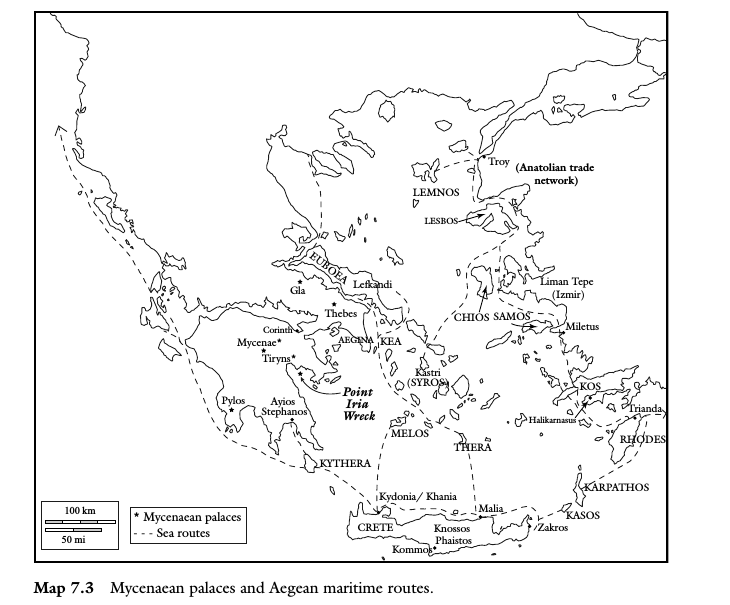
\includegraphics[width=\textwidth]{pottery2.png}
\caption{}
\label{fig:seamap}
\end{figure}

\begin{figure}
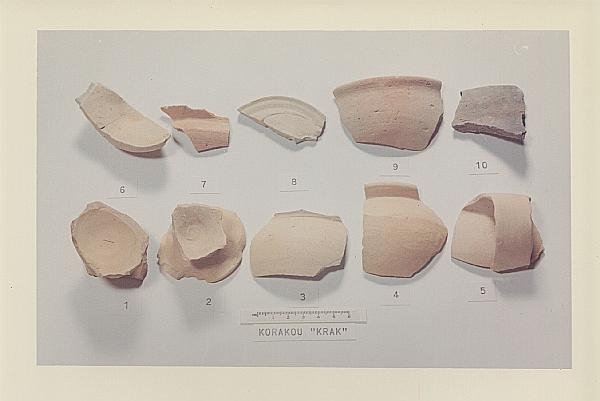
\includegraphics[width=\textwidth]{korakou}
\caption{Example of shreds in the database}
\label{fig:sample}
\end{figure}


\newcommand{\foo}{\hspace{-2.3pt}$\bullet$ \hspace{5pt}}



\begin{figure}
\scalebox{1}{
\begin{tabular}{r |@{\foo} l}
 7000 & Beginning of widespread use of pottery in Mediterranean.
Aegina as maritime center\\
3200-2000 & Early Helladic  \\
3200-2500 &  High point of Anatolian trade network \\
2000-2200 & Disruption of trade between Cyclades, Mainland, and Crete. Upheaval in Mainland \\
2000-1550 & Middle Helladic. Protopalatial and Neopalatial buildings in Crete \\
1650-1500 & Late Helladic I / Late Cycladic I / Late Minoan IA \\
1500-1400 & Late Helladic II \\
1400-1300 & Late Helladic III A \\
1300-1200 & Late Helladic III B. High point of Mycenaean influence on trade\\
1200-1050 & Late Helladic III C \\
1050- & End of Bronze Age. Transitional Period: Argos, Asine and Berbati rise to prominence. 

\end{tabular}
}

\caption{Timeline of Events of Interest (all dates B.C.)}

\label{fig:timeline}
\end{figure}

\section{method}

\printbibliography

\end{document}